\documentclass[12pt,a4paper]{article}
\usepackage[margin=1in]{geometry}
\usepackage{amsmath}
\usepackage{amsfonts}
\usepackage{amssymb}
\usepackage{graphicx}
\usepackage{hyperref}
\usepackage{url}
\usepackage{listings}
\usepackage{listings-rust}

\lstset{language=Rust, style=boxed}

\title{Cyber Physical Robots\\Term Project Progress Report III}
\author{Kanisorn Sangchai (ID: 6538020621)}
\date{October 24, 2025}

\begin{document}

\maketitle

\begin{abstract}
This report presents the third milestone of the Cyber-Physical Robots (CPR) project, which focuses on improving the autonomy and realism of robot coordination. Three main enhancements were introduced: (1) a more reliable exploration and cluster formation process, (2) a message delivery system with variable delay, and (3) a continuous planning and execution mechanism that enables robots to perform multiple pickup and drop-off cycles. The source code for this project is available at: \url{https://github.com/Kanisorn-S/CPR}.
\end{abstract}

\section{Introduction}
This milestone builds upon the previous communication framework by addressing key limitations in robot perception, communication, and task continuity. Earlier, robots that spawned facing walls could not detect gold, message delivery was instantaneous, and robots stopped after a single pickup cycle. To overcome these issues, we improved exploration and cluster formation, introduced randomized message delays, and enabled continuous operation through an iterative task reassignment mechanism.

\section{Exploration and Cluster Finding}
In the previous milestone, each robot relied solely on its initial observation to select a target gold position. As a result, if a robot was spawned facing a wall, it would fail to detect any gold and thus have no target to pursue, rendering it inactive. Additionally, if no other robots shared the same target gold position, that robot would form an empty cluster and remain idle.

To resolve these issues, we implemented two improvements. First, robots are now programmed to rotate randomly until they detect at least one piece of gold. This guarantees that every robot identifies a valid target gold position. Second, we enhanced the cluster formation protocol. Instead of tracking only robots that share the same target gold position, each robot now maintains information about all clusters in the environment. With this knowledge, robots that initially lack a cluster can locate and join other unclustered robots to form a new group. The target gold position for the newly formed cluster is chosen as the one with the highest detected gold amount among its members, as shown in Listing~\ref{lst:singles}. In the case of a tie, a deterministic rule based on the coordinates, shown in Listing~\ref{lst:tie-break}, is applied to decide which position has priority. This ensures that all robots follow identical tie-breaking logic and consistently agree on the same target gold position. A flowchart illustrating the updated cluster formation process is provided in Figure~\ref{fig:cluster-flowchart}.

\begin{lstlisting}[float, caption={Robots without a cluster forming a new group}, label={lst:singles}]
if self.not_received_simple == 0 && self.local_cluster.is_empty() {
  let mut singles = Vec::new();
  let mut max_key: Option<u8> = Some(self.target_gold_amount);
  let mut max_coord: Option<Coord> = self.target_gold;

  for (&(coord, gold_amount), v) in &self.clusters {
    if v.len() == 1 {
      singles.push(v[0]);
      // track max gold amount
    }

    self.local_cluster = singles;
    self.target_gold = max_coord;
    self.consensus_coord = max_coord;
  }
}
\end{lstlisting}

\begin{lstlisting}[float, caption={Rule for breaking ties between coordinates with same gold amount}, label={lst:tie-break}]
pub fn priority(&self, other: Coord) -> bool {
  if self.x > other.x {
    true
  } else if self.x < other.x {
    false
  } else {
    self.y > other.y
  }
}
\end{lstlisting}

\begin{figure}
    \centering
    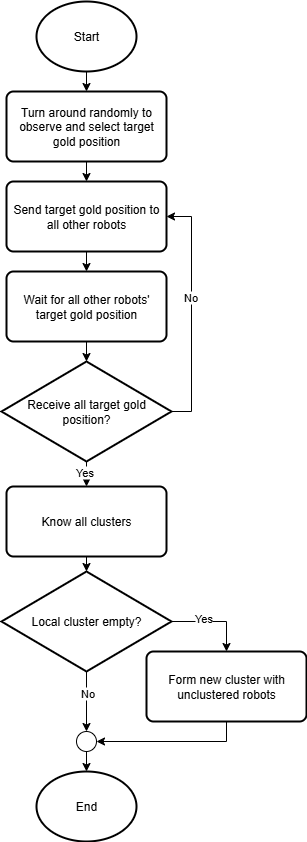
\includegraphics[width=0.5\linewidth]{images/improved_cluster_flow.png}
    \caption{Flow Chart of the Improved Local Cluster Identification Communication Protocol for each Robot}   
    \label{fig:cluster-flowchart}
\end{figure}

\section{Message Arrival Time}
In previous milestones, each robot maintained its own message box. At every simulation step, a robot would randomly select and receive one message from its box. This meant that as long as a message was in the box, it was guaranteed to be received eventually, since one message is processed per step. If the box contained only a single message, that message would be received immediately in the next simulation step. However, this setup still assumed ideal communication, as it did not account for potential message delays caused by real-world factors such as network congestion or interference.

To better reflect realistic communication behavior, we modified the message delivery mechanism. Each message is now assigned a timer with a random value between one and three simulation steps, as shown in Listing~\ref{lst:msg-timer}. When a robot attempts to receive a message, it first checks the timer. If the timer has not yet reached zero, the message cannot be received, and the robot instead decrements the timer, as shown in Listing~\ref{lst:timer-decrement}. This modification introduces variability in message delivery times, providing a more realistic simulation of communication delays. This new message receiving mechanism is illustrated in Figure~\ref{fig:msg-flowchart}.

\begin{lstlisting}[float, caption={Message struct with timer randomly initialized}, label={lst:msg-timer}]
pub struct Message {
  pub sender_id: char,
  pub msg_type: MessageType,
  pub id: u32,
  pub message_content: MessageContent,
  pub timer: u8,
}

impl Message {
  pub fn new(
    sender_id: char, 
    msg_type: MessageType, 
    id: u32, 
    message_content: MessageContent
  ) -> Message {
    let mut rng = rand::rng();
    let timer = rng.random_range(0..=3);
    Self {
      sender_id,
      msg_type,
      id,
      message_content,
      timer,
    }
  }
}
\end{lstlisting}

\begin{lstlisting}[float, caption={New message retrieval mechanism}, label={lst:timer-decrement}]
pub fn retrieve_messages(&mut self) -> Option<Message> {
  if !self.current_messages.is_empty() {
    let mut rng = rand::rng();
    let random_index = rng.random_range(0..self.current_messages.len());
    let random_message = self.current_messages.get_mut(random_index);
    let mut return_message = None;
    let mut message_available = false;
    match random_message {
      Some(message) => {
        if (message.timer == 0) {
          return_message = Some(message.clone());
          message_available = true;
        } else {
          message.timer -= 1;
        }
      },
      None => {}
    }
    if (message_available) {
      self.current_messages.remove(random_index);
    }
    return_message
  } else {
    None
  }
}
\end{lstlisting}

\begin{figure}
    \centering
    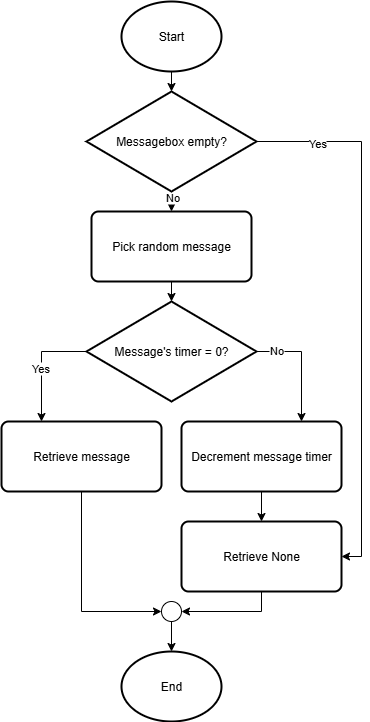
\includegraphics[width=0.6\linewidth]{images/message_flow.png}
    \caption{Flow Chart of the Improved Local Cluster Identification Communication Protocol for each Robot}   
    \label{fig:msg-flowchart}
\end{figure}

\section{Continuous Planning and Execution}
In previous milestones, once a selected pair of robots completed a single pickup and drop-off cycle, they would stop moving entirely. This behavior was undesirable, as the robots should continue operating to collect the remaining pieces of gold in the environment. To resolve this issue, we introduced a continuous planning and execution mechanism. After finishing a pickup and drop-off cycle, the pair of robots now broadcast a \texttt{Done} message to their local cluster, signaling that they are available for new tasks.

Upon receiving the \texttt{Done} message, the cluster assumes the role of a new “global” cluster, as shown in Listing~\ref{lst:new-global}. Each robot within it then broadcasts a new target gold position to the rest of the cluster, leading to the formation of new local clusters within the original one. Each new local cluster goes through the same process as the original local cluster, using PAXOS to nominate a robot pair, picking up, then dropping off a gold bar. This process repeats iteratively, with clusters subdividing after every drop off completion into smaller sub-clusters until a cluster contains only two robots. At that point, the pair is locked together and continues to work cooperatively to collect additional gold. This iterative process is illustrated in Figure~\ref{fig:continuous-flowchart}.
 
\begin{lstlisting}[float, caption={Robot reset after receiving \texttt{Done} message}, label={lst:new-global}]
match message.msg_type {
  MessageType::Done => {
    if !self.received_begin {
      self.received_begin = true;
      self.receiver_ids = self.local_cluster.clone();
      self.local_cluster.clear();
      self.reset();
    }
  }
  // ...
}
\end{lstlisting}

\begin{figure}
    \centering
    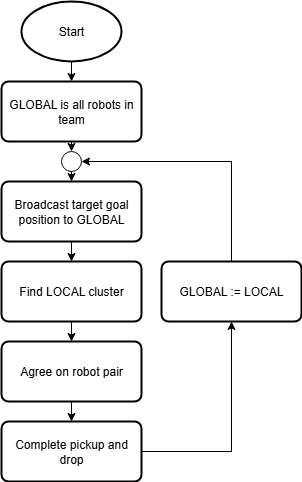
\includegraphics[width=0.6\linewidth]{images/restart.png}
    \caption{Flow Chart of the Continuous Planning and Execution Mechanism}   
    \label{fig:continuous-flowchart}
\end{figure}

\section{Current Progress and Results}
\begin{enumerate}
    \item \textbf{Exploration and Cluster Finding:}  
    Robots now rotate randomly until they detect at least one piece of gold, ensuring all robots identify valid targets. The cluster formation protocol was enhanced so that robots can discover and join others without clusters. Tie-breaking rules ensure consistent agreement on target gold positions.
    
    \item \textbf{Message Arrival Time:}  
    Each message now has a randomized timer between one and three simulation steps before it can be received. This introduces realistic communication delays and variability in message delivery.
    
    \item \textbf{Continuous Planning and Execution:}  
    After completing a drop-off, robot pairs broadcast a \texttt{Done} message to rejoin the cluster and request new tasks. Clusters then reorganize and form new pairs, allowing robots to continuously collect gold without stopping.
\end{enumerate}

\section{Future Work}
\begin{enumerate}
    \item \textbf{Cross Cluster Communication} Currently, robots only communicate within their local clusters. Future work could explore mechanisms for inter-cluster communication to enhance coordination across the entire robot population.
\end{enumerate}

\section{Conclusion}
The third milestone enhances the CPR system with improved autonomy, realistic communication, and continuous operation. Robots can now reliably detect gold, handle communication delays, and sustain their tasks indefinitely, creating a more lifelike and robust cooperative system.

\end{document}